\subsection{Marginal carbon assimilation in a leaf light response}\label{sec:application}

Concavity of a leaf light-response curve means that the marginal gain
in carbon assimilation is nonincreasing with irradiance. We examine
what this assumption contributes to inference from one response sequence
in the Arctic gas-exchange study of \citet{rogers2019arctic}, using
the measurements released by \citet{rogers2019data}. Each record is a
chamber measurement of net assimilation on the same leaf at a specified
incident irradiance. Before fitting either model, we select the smallest
sample identifier in the release, which corresponds to an
Eriophorum angustifolium leaf. The study's quality filters and
exclusion of the dark measurement leave $13$ records over irradiance
$19.1$--$2{,}000.2\,\mu\mathrm{mol}$ quanta $\mathrm m^{-2}\mathrm s^{-1}$.
The measurements were taken in descending illumination over approximately
$37$ minutes, with retained leaf temperatures between $14.1$ and
$15.0\,{}^\circ\mathrm C$.

Let $A(q)$ denote mean net assimilation at irradiance $q$ under the
chamber conditions, measured in $\mu\mathrm{mol}$ $\mathrm{CO}_2$
$\mathrm m^{-2}\mathrm s^{-1}$. We compare the ordinary Gaussian
posterior with its restriction to $\frac{\mathrm{d}^2A}{\mathrm{d}q^2}(q)\leq0$ over the observed
irradiance range. In the scaled coordinate $x=(q-q_0)/d$,
$q_0$ is the midpoint of that range and $d$ its half-width, so the
physical interval becomes $[-1,1]$. The shared model is
\begin{equation}\label{eq:application-model}
\begin{aligned}
 A(q)&=a_0+\sum_{j=1}^{24}a_j\phi_{j,2}((q-q_0)/d),\qquad
 a_0\sim N(0,20^2),\\
 a_j&\overset{\mathrm{ind}}\sim
 N\left(0,\sigma_f^2\sqrt{2\pi}\ell
           \exp(-\ell^2\omega_j^2/2)\right),\\
 y_i\mid A&\overset{\mathrm{ind}}\sim N(A(q_i),\sigma_\varepsilon^2).
\end{aligned}
\end{equation}
The intercept is independent of the other coefficients, and the basis
center is zero in the scaled coordinate. An ordinary Gaussian
marginal-likelihood calculation gives
$\sigma_f=5.625$, $\ell=0.3034$, and $\sigma_\varepsilon=0.3703$,
which both posterior fits use to isolate the effect of the curvature
restriction. The length scale
corresponds to about $301$ irradiance units, and the residual scale has
assimilation units.

The inferential targets are the response $A(q)$, its marginal gain
$\frac{\mathrm{d}A}{\mathrm{d}q}(q)$, and changes in that gain within the observed range.
We report derivatives on the physical irradiance scale, applying factors
$1/d$ and $1/d^2$ to first and second derivatives in the scaled
coordinate. The concavity restriction makes marginal gain
nonincreasing while allowing it to become negative, and imposes no
finite saturation level beyond the fitted interval.

We fit the concave model by applying the convexity sampler to $-A$
and the negated responses, and obtain the unconstrained comparison by
direct Gaussian simulation. Sampling settings, convergence diagnostics,
and posterior predictive assessment are given in the
supplementary material.

The response and derivative panels in \cref{fig:light-response} show
different effects of the constraint. Posterior mean responses are close
at many observed irradiances, but the unconstrained marginal gain can
increase within the range and has substantially wider pointwise intervals
at high irradiance. Concavity imposes nonincreasing marginal gain
on each posterior curve, so the ordering holds for the individual
curves whose uncertainty the right panel summarizes.
\begin{figure}[H]
\centering
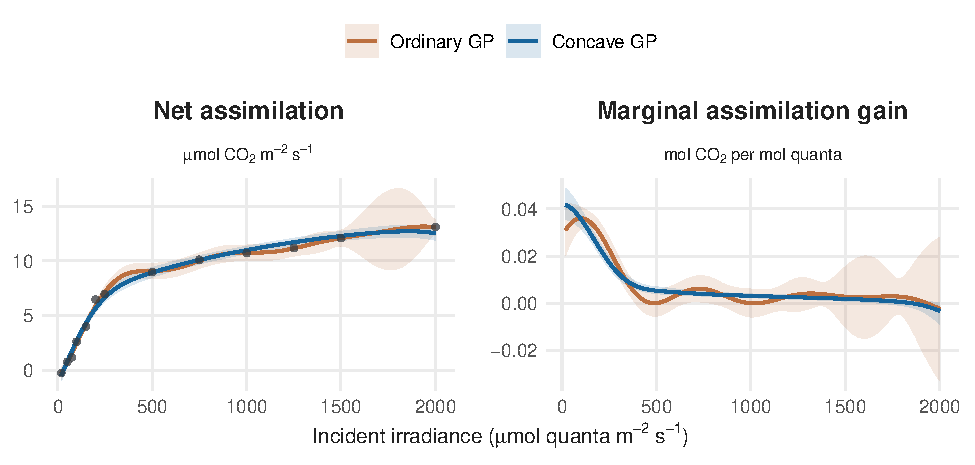
\includegraphics[width=\textwidth]{figures/light_response.pdf}
\caption[Leaf light-response comparison]{Posterior comparison for $13$
net assimilation measurements from one Arctic
Eriophorum angustifolium leaf. The left panel shows net
assimilation in $\mu\mathrm{mol}$ $\mathrm{CO}_2$
$\mathrm m^{-2}\mathrm s^{-1}$, with observations in black.
The right panel shows its derivative with respect to incident irradiance,
in $\mathrm{mol}$ $\mathrm{CO}_2$ per mol quanta.
Orange and blue lines are ordinary Gaussian and concavity-conditioned
posterior means, with shaded pointwise $95\%$ equal-tail credible
intervals for the latent quantities. Both fits use the same covariance
and noise parameters and the same rank-$24$ HSGP expansion.}
\label{fig:light-response}
\end{figure}

\cref{tab:application} gives selected response and derivative summaries.
For example, the assimilation increase from $500$ to $1{,}500$
irradiance units has concave posterior mean \AppGainMean\ and
$95\%$ equal-tail interval $(\AppGainLower,\AppGainUpper)$.
The corresponding unconstrained mean is \OrdGainMean\ with interval
$(\OrdGainLower,\OrdGainUpper)$, all in assimilation units.
The $95\%$ intervals for the difference in marginal gain between $100$
and $1{,}500$ are positive under both fits, so the ordinary Gaussian
analysis already supports diminishing gain for this pair of irradiances.
Conditioning extends that ordering to the entire interval while reducing
posterior uncertainty about marginal gain at high irradiance.
\begin{table}[htbp]
\centering
\small
\begin{tabular}{lrr}
\toprule
Quantity & Unconstrained & Concave \\
\midrule
$A(100)$ & 2.46 (2.11, 2.80) & 2.67 (2.38, 2.97) \\
\addlinespace[2pt]
$A(500)$ & 9.08 (8.38, 9.78) & 8.92 (8.49, 9.38) \\
\addlinespace[2pt]
$A(1{,}500)$ & 12.08 (11.36, 12.80) & 12.27 (11.86, 12.70) \\
\addlinespace[2pt]
$\dfrac{\mathrm{d}A}{\mathrm{d}q}(100)$ & 0.0361 (0.0315, 0.0407) & 0.0357 (0.0316, 0.0399) \\
\addlinespace[2pt]
$\dfrac{\mathrm{d}A}{\mathrm{d}q}(1{,}500)$ & 0.0029 (-0.0099, 0.0155) & 0.0019 (0.0010, 0.0028) \\
\addlinespace[2pt]
$\dfrac{\mathrm{d}A}{\mathrm{d}q}(100)-\dfrac{\mathrm{d}A}{\mathrm{d}q}(1{,}500)$ & 0.0332 (0.0197, 0.0467) & 0.0338 (0.0295, 0.0381) \\
\addlinespace[2pt]
$A(1{,}500)-A(500)$ & 3.00 (2.00, 4.01) & 3.35 (2.73, 3.99) \\
\bottomrule
\end{tabular}

\caption[Response and marginal-gain summaries]{Posterior means with
pointwise $95\%$ equal-tail credible intervals for the leaf light-response
model in \cref{eq:application-model}, with arguments measured in
$\mu\mathrm{mol}$ quanta $\mathrm m^{-2}\mathrm s^{-1}$.
Response values and their differences have units
$\mu\mathrm{mol}$ $\mathrm{CO}_2$ $\mathrm m^{-2}\mathrm s^{-1}$,
while derivatives and their difference have units mol $\mathrm{CO}_2$
per mol quanta. Both columns use the same covariance and noise
estimates, with the concave column additionally conditioning on
nonpositive curvature throughout the observed range.}
\label{tab:application}
\end{table}

The upper endpoint also reveals the limits of a physiological
interpretation. Only \AppEndpointPercent\ of concave draws have a
nonnegative slope at the highest measured irradiance, even though
assimilation increases between the two highest observed irradiances.
The inferred decline near the endpoint depends on the curvature
restriction and stationary prior, and cannot by itself establish
photoinhibition in this leaf.

The example illustrates how a stipulated curvature restriction changes
derivative inference for one sequence, whose observation frame does
not support conclusions about dark respiration or a species response.
Likewise, the analysis does not establish an irradiance optimum
independently of the shape assumption.
